\section{Where the symmetry tax lives}
\label{sec:structure}

\paragraph{The mirror operator.}
Let $x_l \in \mathbb{R}^{T\times d}$ be the $T$ tokens of an image at layer $l$ of the residual stream, and
$\tilde{x}_l$ the tokens of its mirror image, with the patch grid flipped back so that each token is compared with the
token at the same image position. If the network treated an image and its mirror image alike up to a change of basis,
we would have $\tilde{x}_l \approx x_l A_l$ for an orthogonal matrix $A_l$ with $A_l^2 = I$. The least-squares fit has
a closed form: with $C_l = \sum x_l^\top \tilde{x}_l$ summed over tokens and images and
$\tfrac12(C_l + C_l^\top) = V \Lambda V^\top$,
\begin{equation}
  A_l = V \,\mathrm{sign}(\Lambda)\, V^\top .
  \label{eq:operator}
\end{equation}
The $+1$ eigenvectors of $A_l$ span the \emph{even} directions of the stream, which a mirror leaves unchanged, and the
$-1$ eigenvectors span the \emph{odd} directions, which change sign; we write $d_+$ and $d_-$ for their numbers.

\paragraph{Twins and the tax.}
Two hidden neurons $i$ and $j$ of an MLP are \emph{twins} when neuron $j$ fires on the mirrored image where neuron $i$
fires on the original. We pair neurons by a maximum-weight matching on the correlation between neuron $i$ on mirrored
images and neuron $j$ on the originals; unmatched neurons are their own twins. We call a pair \emph{strong} when this
correlation is at least 0.5. An MLP is exactly mirror-equivariant when its weights satisfy $P W_1 = W_1 A_l$ and
$A_{l+1} W_2 = W_2 P$, where $P$ swaps twins. The \emph{tax} of a layer is the share of its weights that this
constraint makes redundant, $1 - (\text{free parameters})/(\text{dense parameters})$, with the count of
Section~\ref{sec:method}.

\paragraph{How close the weights are.}
To measure how close a trained MLP is to this form, we project each weight matrix onto it and record the share of its
energy that the projection removes, $s = \lVert W - W_{\mathrm{eq}} \rVert_F^2 / \lVert W \rVert_F^2$. A random
structure of the same size (a random mirror operator with the same $d_+$ and a random pairing with the same number of
twins) also removes energy, about 48\% in the first block of DINOv2-B/14 with registers, so we report the \emph{ratio
to null}: $s$ divided by its mean over 20 random structures. A ratio of 1 means the weights are no closer to the
fitted structure than to a random one, and lower means closer. For example, the first block of DINOv2-B/14 with
registers loses 27\% (first MLP layer) and 20\% (second) of its weight energy to the projection, so it is far from
random but not exactly symmetric. The same procedure, with the matching token map, measures up-down mirroring (UD),
180-degree rotation (R180) and 90-degree rotation (R90, with four-cycles of neurons).

\paragraph{Models.} We measure 14 released models: five DINOv2 models (four sizes with registers and the base size
without)~\citep{oquab2024dinov2,darcet2024registers}, DeiT~III~\citep{touvron2022deit}, DINO~\citep{caron2021emerging},
DINOv3~\citep{simeoni2025dinov3}, EVA-02~\citep{fang2024eva}, MAE~\citep{he2022masked},
CLIP~\citep{radford2021learning}, SigLIP~2~\citep{tschannen2025siglip}, and two CNNs, ConvNeXt~\citep{liu2022convnet}
and ResNet-50~\citep{he2016deep}. All structures are fitted on 2{,}000 ImageNet training images.

\begin{figure}[t]
  \centering
  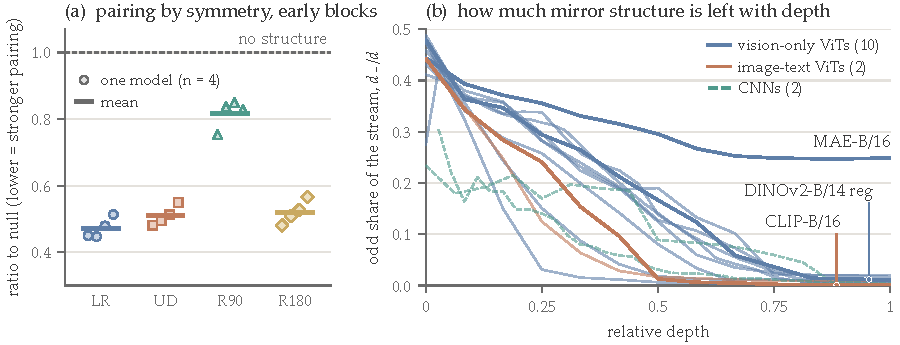
\includegraphics[width=\linewidth]{figures/fig_symmetry_depth.pdf}
  \caption{\textbf{Where mirror structure lives.} (a) Ratio to null of four symmetries in the first half of the
  blocks of four models (DINOv2-B/14 with and without registers, DINOv2-L/14 with registers, DeiT~III-B/16); lower is
  closer to the symmetric form, 1 is no closer than a random structure. Markers are models, bars are means. (b) Share
  of odd directions in the residual stream, $d_-/d$, against relative depth, for 14 models.}
  \label{fig:symmetry}
\end{figure}

\paragraph{The tax lives in the early blocks.}
In every model, mirror structure is concentrated in the first half of the network (Figure~\ref{fig:symmetry}b). At the
input of the first block, 330 to 380 of the 768 stream directions are odd in every ViT-B model; at the output of the
last block, 11 of our 12 transformers have at most 13 odd directions left, so their deep features are almost unchanged
by a mirror. MAE is the exception and keeps 191. Twins follow the same pattern: in DINOv2-B/14 with registers the
matching pairs 1{,}168 of the 1{,}536 possible pairs in the first MLP and 17 in the last, and tying the twins of the
first six blocks would remove 42\% of their MLP weights. In the first half, left-right structure is far from random
in all 14 models, with ratios to null between 0.42 and 0.62 for 13 of them, including the two CNNs. The exception,
DINOv2-g (0.77), and EVA-02 (0.62) are the two models with gated SwiGLU MLPs, and they form few strong twins
(Appendix~\ref{app:structure}); a gated unit can itself be odd, so it need not pair. In late blocks the ratio to null
is often lower than in early blocks, but this reflects how little structure is left there: with almost no odd
directions and few twins, the fitted and the random structures both remove very little energy.

\paragraph{Early structure is not specific to left-right flips or to flip augmentation.}
We expected the early structure to be specific to left-right flips and to the flip augmentation used in training;
four pre-registered predictions to that effect failed (MUST-04 P4.1 to P4.3 and CORE-04 P4.2,
Appendix~\ref{app:prereg}). In the four models where we
measured all four symmetries, up-down mirroring gives almost the same ratio to null as left-right mirroring (mean 0.51
against 0.47), while 90-degree rotation is much weaker (0.82; Figure~\ref{fig:symmetry}a). Rotation by 180 degrees,
which is a left-right flip followed by an up-down flip, also gives 0.52. None of these models was trained with
vertical flips or with 90- or 180-degree rotations. Nor does the early structure need flip augmentation: CLIP, whose
only augmentation is a random crop~\citep{radford2021learning}, has a left-right ratio of 0.51, within the range of the
flip-trained models, and DINOv3, whose released teacher configurations switch flips off (the configuration of the
ViT-B student is not public), has 0.45. Both differ from the other models in more than augmentation, so this is
evidence, not proof.

One explanation, which we formed after these predictions failed, fits the observations. The power spectrum of any
real image is unchanged by a 180-degree rotation, so a left-right flip and an up-down flip change it in exactly the
same way: the power spectrum cannot tell the two mirrors apart. A 90-degree rotation maps one orientation onto
another, and the power of natural images varies with orientation~\citep{vanderschaaf1996modelling,%
torralba2003statistics}; we would expect horizontal and vertical structure to differ in particular, since gravity gives
real scenes horizons and upright objects. Early features are local, and a patch filter shared across positions sees
statistics pooled over the image. If such features are shaped mainly by second-order statistics, and the visual world
has no preferred handedness, they should carry left-right and up-down pairing to a similar degree and 90-degree
pairing much less, whatever the augmentation. Deeper features encode layout, for which up and down are not
interchangeable: up-down structure fades with depth in all 14 models and 180-degree structure in all four where we
measured it (Appendix~\ref{app:structure}). We have not tested this explanation causally.

Late blocks hold little mirror structure to collect, but in a residual network they must share the stream's mirror
operator with the early blocks if the whole model is to be exactly equivariant. The next section builds the conversion
on this constraint.
